\section{Metrics}
\label{sec:Solution} 

 \autoref{fig:Metrics_shot} provides an overview of the requirements engineering (RE) and development processes (SE), explaining the metrics graphically. The work flow is divided into stages (milestones) along the time-line: t1,t1',t2...ti'.
 Output of every RE stages is an RE Artifac: the document with the textual elaborated requirements, i.e., analysed, structured, corrected and so on. It means, that the first stage of the RE process brings the changes into initial "raw" requirements.
 
 Netx step is to provide this RE artifac to  software engineers.
 
 Bz this metrics we consider 


%\begin{figure}[htpb!]
%	\centering
%		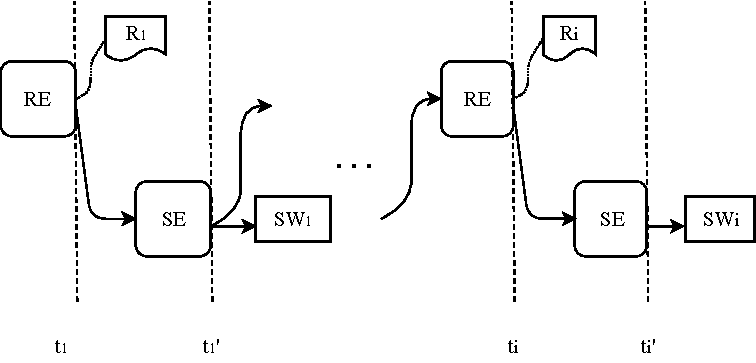
\includegraphics[width=0.5\textwidth]{Metrics_shot.pdf}
%	\caption{metrics explanation}
%	\label{fig:Metrics_shot}
%\end{figure}

\begin{figure}[!t]
	\centering
		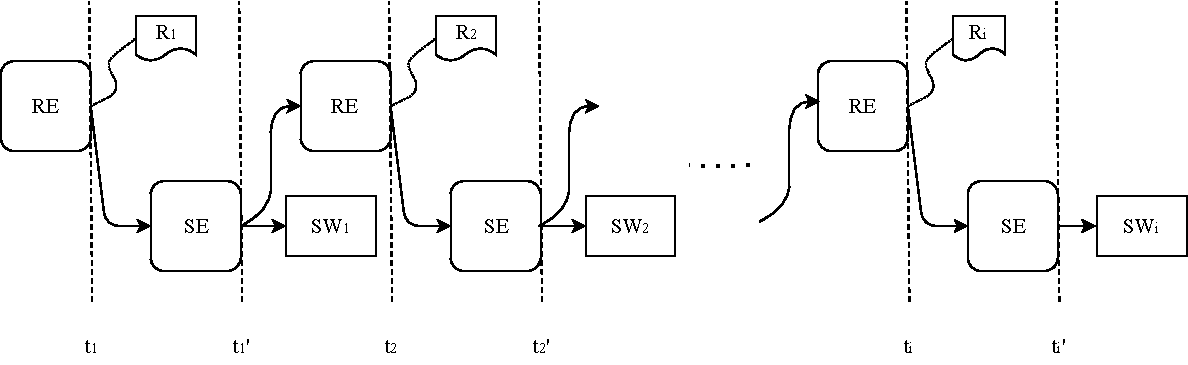
\includegraphics[width=0.5\textwidth]{MetricsDiag.pdf}
	\caption{metrics explanation}
	\label{fig:Metrics_shot}
\end{figure}


$\mu_{1}(R_{j}) = i-j$

$\mu_{2}(R_{j}) = t_{i}-t_{j}$

$\mu_{3}(R_{j}) = \displaystyle\sum_{j} t_{j+1}-t_{j}\acute{}$

$\mu_{4} = \displaystyle\sum_{j} (t_{j+1}-t_{j}\acute{} + p_{j}*(t_{j}\acute{} - t_{j}))$


